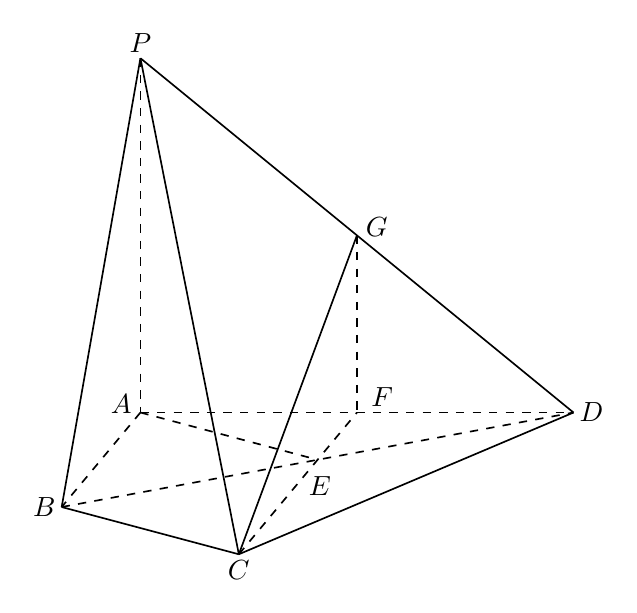
\begin{tikzpicture}[x=1cm,y=1cm,font=\normalsize,
  edge/.style={draw=black,solid,line width=.6pt},
  hide/.style={draw=black,dashed,line width=.6pt}]
% Quadrangular pyramid P-ABCD, F on AD, G midpoint of PD, E interior
\coordinate (P) at (1.0000000000,6.0000000000);
\coordinate (A) at (1.0,1.5);
\coordinate (B) at (0.0,0.3);
\coordinate (C) at (2.2500000000,-0.3000000000);
\coordinate (D) at (6.5,1.5);
\coordinate (F) at (3.7500000000,1.5000000000);
\coordinate (G) at (3.7500000000,3.7500000000);
\coordinate (E) at (3.2500000000,0.9000000000);
% solid pyramid edges and base front
\draw[edge] (P)--(B);
\draw[edge] (P)--(C);
\draw[edge] (P)--(G);
\draw[edge] (G)--(D);
\draw[edge] (B)--(C);
\draw[edge] (C)--(D);
\draw[edge] (C)--(G);
% hidden: PA, base back, diagonals, GF
\draw[hide] (P)--(A);
\draw[hide] (A)--(D);
\draw[hide] (A)--(B);
\draw[hide] (A)--(E);
\draw[hide] (B)--(D);
\draw[hide] (C)--(F);
\draw[hide] (G)--(F);
\node[above,inner sep=2pt] at (P) {$P$};
\node[left,inner sep=2pt,xshift=-1pt,yshift=3pt] at (A) {$A$};
\node[left,inner sep=2pt] at (B) {$B$};
\node[below,inner sep=2pt] at (C) {$C$};
\node[right,inner sep=2pt] at (D) {$D$};
\node[below left,inner sep=2pt,xshift=7pt,yshift=-4pt] at (E) {$E$};
\node[above right,inner sep=2pt,xshift=3pt] at (F) {$F$};
\node[right,inner sep=2pt,xshift=1pt,yshift=3pt] at (G) {$G$};
\end{tikzpicture}
